\documentclass{lni}


%\IfFileExists{latin1.sty}{\usepackage{latin1}}{\usepackage{isolatin1}}
\usepackage[latin1]{inputenc}
% Verwenden von T1 Fonts
\usepackage[T1]{fontenc}
\usepackage[ngerman]{babel}
\usepackage{graphicx}
\usepackage{amsmath}
\usepackage{amssymb}
\usepackage{listings}
%\usepackage{hyperref}
\usepackage{fancyvrb}
\usepackage{color}
\usepackage{algorithmic}
\usepackage{algorithm}
\usepackage{float}

\floatstyle{ruled}
\newfloat{program}{H}{lop}
\floatname{program}{Listing}
\include{syntax}
\usepackage{lastpage}
\thispagestyle{plain}
\pagenumbering{arabic}


\author{
	Lusy \\
	\\
	%Abteilung \\
	Freie Universit�t Berlin \\
	%Anschrift \\
	%Postleitzahl Ort \\
	emaiaddresse@autor1 
}
\title{Semantische Modellierung von mathematischen Publikationen und Definition eines geeigneten �hnlichkeitsma�es}

\newtheorem{mdef}{Definition}
\begin{document}
\maketitle

\begin{abstract}
lala
\end{abstract}

\tableofcontents
\newpage
%-------------------------------------------------------
%----Hauptteil------------------------------------------
%-------------------------------------------------------

%\section{Einleitung}

\subsection{Motivation}
Titel, Thema, Autor, Erscheinungsjahr, Journal und Literaturverweise sind nur einige f�r eine wissenschaftliche Publikation relevante Metadaten.
Diese stehen in bestimmten Relationen zueinander.
Es gibt schon mehrere Repr�sentationen von wissenschaftlichen Arbeiten: Zitations- oder Koautorgraphen ber�cksichtigen aber beispielsweise nur Referenzen oder Autoren.
Zus�tzliche Metadaten k�nnen jedoch f�r eine Analyse ebenfalls bedeutende und interessante Einsichten bringen.
Durch den Aufbau eines semantischen Netzes, das alle zu einer Publikation relevanten Informationen enth�lt, soll ein allgemeineres Modell f�r wissenschaftliche Publikationen entwickelt werden.
Durch die Ber�cksichtigung der in diesem Modell erfassten semantischen Relationen wird dann versucht, ein m�glichts pr�zises �hnlichkeitsma� f�r wissenschaftliche Publikationen zu entwerfen. %vlt beispiele (A ist Autor von Paper P, P ist Journal C erschienen, hat X,Y,Z als Keywords usw)
Ein gutes �hnlichkeitsma� findet mehrere Gebr�uche: es kann bei automatischer Klassifizierung von Arbeiten in einer wissenschaftlichen Datenbank oder als Ausgangspunkt f�r das Vorschlagen verwandter/relevanter Dokumente eingesetzt werden.
Fr�here Entw�rfe von �hnlichkeitsma�en beziehen nur bibliometrische Kategorien wie Zitationsanalysen (von direkten Zitaten, Kozitationen oder bibliographischen Kopplungen) oder Koautorenschaften ein \cite{Kessler:1963} \cite{Small_1973} \cite{DBLP:journals/corr/abs-1109-1059}.%referenz!
Indem alle Metadaten zu einer Publikation und ihre semantische Erfassung in eine neue Definition integriert werden, sollen genauere Ergebnisse erzielt werden.


% themabeschreibung (vlt mit beispiel)
% und wir wollen das machen, weil... (warum ist die frage wichtig/interessant)
% forschungszusammenhang: was gibts schon zum thema, was ist das neue


\subsection{Zielsetzung}
% define keywords/schl�sselkonzepte
% Was will ich damit erreichen/ Welche Ergebnisse strebe ich an?
% Datensatz
% Verfahren
% benutzte Werkzeuge

Ziel dieser Arbeit ist es ein semantisches Netz zu modellieren, das alle zu einer mathematischen Publikation relevanten Metadaten ber�cksichtigt und mathematische Publikationen zueinander in Relation stellt.
Im zweiten Teil der Arbeit wird dieses Netzwerk als Grundlage f�r die Formulierung eines �hnlichkeitsma�es und �hnlichkeitsanalysen verwendet.
Das vorgeschlagene �hnlichkeitsma� wird in Anlehnung an den schon existierenden Ma�en SimRank \cite{simrank2002}, P-Rank \cite{ZhaoHS09} und C-Rank \cite{DBLP:journals/corr/abs-1109-1059} rekursiv definiert.
Hierbei werden nicht nur Zitationen, sondern auch andere semantische Relationen zwischen einer Publikation und ihren einzelnen Metadaten, wie z.B Autor, Quelle, Erscheinungsjahr und Keywords, gez�hlt.
%wie sieht es aus?
Die Qualit�t des definierten �hnlichkeitsma�es wird ermittelt, indem die Ergebnisse, die es liefert, mit der schon im Datensatz durch Fachexperten vergebenen MSC-Klassifizierung
\footnote{Die Mathematical Subject Classification (MSC) ist eine Klassifizierungskonvention, die durch die wissenschaftlichen Datenbanken Mathematical Reviews und das Zentralblatt Mathematik genutzt wird. F�r den Aufbau siehe http://www.ams.org/mathscinet/msc/msc2010.html} verglichen werden.
\\
Der der Ausarbeitung zugrundeliegende Datensatz beinhaltet die Metadaten und MSC-Klassifikationen von ca. $2,900,000$ Publikationen vom Zentralblatt Mathematik, FIZ Karlsruhe.
%wie wird das �hnlichkeitsma� definiert/evaluiert (Verfahren + Werkzeuge)

\subsection{Aufbau der Arbeit}

Im Weiteren wird diese Arbeit folgenderma�en aufgebaut:
\\
Kapitel 2 stellt die theoretischen Grundlagen der Bibliometrie vor, beschreibt semantische Netzwerke als eine M�glichkeit der Wissensrepr�sentation und stellt Zusammenh�nge zu schon vorhandenen Studien her.
In Kapitel 3 werden die Eigenschaften und Besonderheiten vom zmath-Datensatz, das modellierte semantische Netz, sowie die Abbildung der Metadaten auf das entworfene Schema betrachtet und ein �hnlichkeitsma� f�r mathematische Publikationen definiert.
In Kapitel 4 untersucht den zugrundeliegenden Datensatz auf �hnlichkeiten mit Hilfe des bereits erarbeiteten �hnlichkeitsma�es und stelle eine detaillierte Auswertung der erzielten Ergebnisse dar.
Kapitel 5 gibt einen Ausblick und schl�gt Ans�tze f�r weiterf�hrende Untersuchungen vor und fasst nochmal abschlie�end die Arbeit zusammen.

%-present the subject, it could be with an example
%-define the important words
%-present the hypothesis + arguments etc.
%-describe how the body is organized

%Quite literally, the Introduction must answer the questions, "What was I studying? Why was it an important question? What did we know about it before I did this study? How will this study advance our knowledge?"


%\section{Grundlagen}
% Vlt Reihenfolge von Bibliometrie und Semantische Netzwerke umdrehen

\subsection{Bibliometrie}
% Ganz kurz was ist die Bibliometrie, Forschungsschwerpunkt
% Was sind wichtige Parameter/Kenngr��en, die f�r uns relevant sind/wir verwenden
% was sind die Kritikpunkte dran/ Warum glaube ich, dass diese Kenngr��en alleine nicht genug sind, um �hnlichkeit zu definieren

Die untersuchte Problemstellung, die angewandten Methoden oder die Kombination von beiden m�ssen bei einer wissenschaftlichen Arbeit neu sein, damit diese in ihrem Forschungsfeld einen Mehrwert hat.
Frank Havemann beschreibt Bibliometrie als die Disziplin, die nachweisbare und ad�quate Methoden anbietet, um diese Aufgabe zu l�sen \cite{frank2009einfuehrung}.
Ferner wird Bibliometrie als ein Versuch, ``Ordnung im heutigen Informationsflut zu schaffen'' bezeichnet \cite{NAB2004} .
Rafael Ball und Dirk Tunger schlagen folgende Definition vor: ``Anwendung mathematischer und statistischer Methoden zur Erkl�rung der Prozesse von schriftlichen Mitteilungen'' \cite{bibliogrundw2005}.
\\
\\
Der Begriff $Bibliometrie$ existiert seit 1969 und ist auf A. Pritchard zur�ckzuf�hren, auch wenn die ersten bibliometrischen Analysen schon bereits am Anfang des 20. Jahrhunderts durchgef�hrt wurden.
Diese versuchen die Wahrnehmung von Facharbeiten, den Einfluss einzelner Autoren (oder Publikationen), ihre Integration in der entsprechenden Forschungsgemeinschaft und ihre internationale Pr�senz aufzuzeigen.
Es werden unter Anderem folgende Gegenst�nde quantitativ untersucht: die Trendentwicklung der Forschungsschwerpunkte einer bestimmten wissenschaftlichen Disziplin, die Produktivit�t, die Resonanz oder den Einfluss eines Autors, einer Forschergruppe oder eines Forschungsinstituts, die Internationalit�t und die Kooperationsbereitschaft auf einem bestimmten Forschungsfeld.
Die mit den bibliometrischen Methoden gewonnenen Erkenntnisse sind oft Ausschlag gebend bei neuen Literaturbeschaffungen in Bibliotheken, oder werden als Ausgangspunkt f�r eine leistungsorientierte Mittelvergabe in Wissenschaft und Forschung eingesetzt.
\\
\\
Die gegenw�rtige Tendenz, diese statistischen Verfahren alleine f�r das Treffen dieser Entscheidungen zu benutzen, wird allerdings von diversen Experten stark kritisiert.
Sie vertreten die Meinung, dass Forschung viel zu wichtig ist, um nur mit Hilfe von einem einzigen, zudem so vagen, Werkzeug, bewertet wird.
Statistische Daten erscheinen objektiver und unabh�ngiger als manche anderen Praxen, wie z.B. Peer-Reviews \cite{citationstats2008}.
Die Experten geben zu, dass es verlockend ist, eine einfache und einfach me�bare Vergleichsbasis f�r verschiedene Publikationen, Journalen, Wissenschaftlerinnen, etc. zu haben.
Sie warnen aber vor, dass Zahlen nicht immer einer n�chternen Beurteilung �berlegener sind, leicht falsch interpretiert werden k�nnen und mit Vorsicht zu genie�en sind \cite{citationstats2008}.
Dennoch werten diese Mathematiker und Statistiker die Bibliometrie nicht als komplett falsch oder nutzlos, sondern raten dazu, f�r etliche Auswertungen, die bibliometrischen Methoden mit anderen Verfahren zu kombinieren.
An der Stelle werden zwei von den Unterthemen der Bibliometrie kurz umrissen, die auch in die Definition von �hnlichkeitsma�, die diese Arbeit anbietet, in gewisser Hinsicht einflie�en werden.
%warum
\\

\subsubsection{Zitationsanalyse}

Die Zitationsanalyse ist eines der Kerngebiete der Bibliometrie.
Sie untersucht die Beziehungen zwischen wissenschaftlichen Arbeiten aufgrund der Z�hlung von im Literaturverzeichnis angegebenen Quellen.
% Kritik
% Bilder!!!
\\
\\
Eine spezielle Relation, die auf Zitationen basiert, ist die bibliographische Kopplung.
Zwei Publikationen werden als bibliographisch gekoppelt bezeichnet, wenn sie ein gemeinsames fr�heres Werk zitieren (Abbildung \ref{fig:bibcoupling}).

Die bibliographische Kopplung ist ein n�tzlicher Indikator, um Beziehungen zwischen frisch publizierten Arbeiten herzustellen, bzw. zwischen Artikeln, die in einem geringen zeitlichen Abstand publiziert worden sind.
Mehrere Studien kennzeichnen zwei Publikationen desto �hnlicher, je st�rker bibliographisch gekoppelt diese sind (d.h. je mehrere gemeinsamen Quellen diese zitieren).%Quellen!!
\begin{figure}
    \begin{subfigure}[h]{0.5\textwidth}
        \centering
        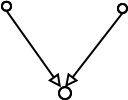
\includegraphics[scale=0.5]{./diagrams/bibliographic_coupling.png}
        \caption{Bibliographische Kopplung: Publikationen 1 und 2 sind bibliographisch gekoppelt, weil sie beide Publikation 3 zitieren}
        \label{fig:bibcoupling}
    \end{subfigure}
    \qquad
    \begin{subfigure}[h]{0.5\textwidth}
        \centering
        \includegraphics[scale=0.5]{./diagrams/co-citation.png}
        \caption{Kozitation: Publikationen 1 und 2 stehen in einer Kozitation-Relation zu einander, weil sie beide durch Publikation 3 zitiert werden}
        \label{fig:cocitation}
    \end{subfigure}
    \caption{Zitationsrelationen}
    \label{fig:citrelations}
\end{figure}
\\
\\
Eine andere Zitationsrelation ist die Kozitation.
Eine Kozitation von zwei oder mehreren Arbeiten liegt vor, wenn alle diese von einer dritten gemeinsam zitiert werden (Abbildung \ref{fig:cocitation}).
%Henry Small!!
Laut Kim und Barnett \cite{DBLP:conf/amcis/KimB08} werden Cluster von h�ufig kozitierten Dokumenten als stark zusammenh�ngend betrachtet.
% "Clusters of highly co-cited documents are considered to have high mutual dependance"\cite{DBLP:conf/amcis/KimB08}
\\
\\
\begin{figure}[h]
    \centering
    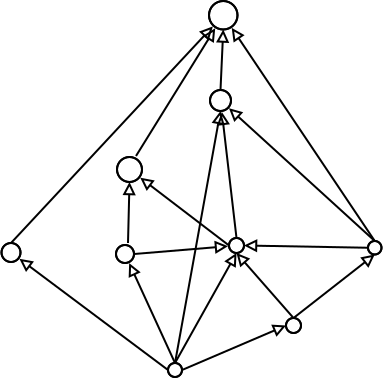
\includegraphics[scale=0.5]{./diagrams/citation_network.png}
    \caption{Beispiel f�r ein Zitationsnetzwerk}
    \label{fig:citenetwork}
\end{figure}
Aufgrund dieser beiden Auspr�gungen von Zitationsrelationen und auch noch der einfachsten und naheliegendsten: dem direkten Zitat, werden Zitationsnetzwerke aufgebaut.
Das sind Graphen, deren Knoten f�r Publikationen stehen und wo jede Kante eine Zitation veranschaulicht (Abbildung \ref{fig:citenetwork}).
Auf der Basis von Zitationsnetzwerken k�nnen Cluster von eng zusammenh�ngenden Dokumenten ermittelt werden.
Die gerichteten Kanten eines solchen Graphen stehen auch f�r eine zeitliche Richtung - das zitierte Paper ist stets �lter als die Arbeit, von der es zitiert wird.
Viele Experten schlagen �hnlichkeitsma�e vor, die auf Zitationsnetzwerke beruhen (siehe \cite{simrank2002}, \cite{evalpubsim2005}, \cite{Small_1973}, \cite{ZhaoHS09}, \cite{DBLP:journals/corr/abs-1109-1059}.
\\
\\
Auch wenn diese bibliometrisch bibliometrische Herangehensweise als ein sinnvoller erster Ansatz erscheint, um die �hnlichkeit zwischen zwei wissenschaftlichen Arbeiten zu ermitteln, werden bei n�herer Betrachtung mehrere Probleme/Kritikpunkte aufgedeckt, weswegen auf jeden Fall auch andere �hnlichkeitsindikatoren gesucht werden m�ssten:\\
\begin{itemize}
\item Selbstzitate: die Menschen tendieren dazu, sich selbst oder andere, die sie kennen und mit denen sie zusammen gearbeitet haben, �fters zu zitieren \cite{DBLP:conf/amcis/KimB08} \cite{frank2009einfuehrung}.
Dadurch versuchen sie einerseits ihre eigenen Parameter, wie z.B. Rankings aufgrund von Zitationszahlen, andererseits auch diese von Kollegen, Bekannten, etc. zu verbessern (die so genannten ``Dankbarkeits-'' oder ``Gef�lligkeitszitate'') \cite{DBLP:conf/isiwi/Schlogl00}.
Dazu kommt auch noch der Druck von Herausgebern von Journalen, dass Arbeiten, die in einem bestimmten Journal publiziert werden, m�glichst h�ufig andere Ver�ffentlichungen von diesem Journal zitieren (wieder aufgrund von Verbesserungen von bestimmten bibliometrischen Parametern) \cite{frank2009einfuehrung}.
\item Zitate von Standardwerken (sogenannten ``Authorities'') oder �bersichtsartikeln kommen vergleichsweise �fter vor und m�ssen mit Vorsicht genossen werden \cite{DBLP:conf/isiwi/Schlogl00} \cite{evalpubsim2005}.
\item Es dauert, bis sich eine Arbeit etabliert hat, deshalb werden fr�here Werke �fters zitiert \cite{DBLP:conf/isiwi/Schlogl00}.
\item Papers, die auf anderen Sprachen als Englisch ver�ffentlicht werden, werden tendenziell seltener gelesen und weniger zitiert \cite{Bornmann08}.
\item Manchmal werden Zitate einfach weggelassen \cite{DBLP:conf/isiwi/Schlogl00}.
\item Zwei Arbeiten, die eine Dritte zitieren, k�nnen sich wom�glich auf komplement�re Aspekte davon beziehen.
\item Artikel mit langen Referenzlisten sind tendenziell st�rker bibliographisch gekoppelt als solche mit kurzen Listen, wenn man nur die Anzahl der zusammen zitierten Arbeiten z�hlt \cite{frank2009einfuehrung}.
\item Zitate, die andere Arbeiten referenzieren, ohne das Originalwerk zu konsultieren: es werden in Bibliographien �fters Arbeiten aus dem Literaturverzeichnis eines zitierten Dokuments entnommen \cite{DBLP:conf/isiwi/Schlogl00}.
\item Rechtschreibfehler in Zitaten: aufgrund deren kann das zitierte Werk nicht eindeutig bestimmt/wiedergefundnen werden, was das Zitat wertlos macht \cite{Bornmann08}.
% Ansatz zur Normalisierung relative bibliographische Kopplung (Jaccard- und Salton-Index), messen die Kopplung bezogen auf die L�nge der Referenzlisten
\end{itemize}

\subsubsection{Koautorenschaft}

Der zweite Schwerpunkt, der hier noch kurz umrissen wird, ist die Koautorenschaft.
Als Koautoren werden zwei oder mehrere Wissenschaftler oder Wissenschaftlerinnen bezeichnet, die gemeinsam eine Arbeit ver�ffentlicht haben.
Koautorenschaft wird auch oftmals als ein �hnlichkeitskennzeichen gewertet. %Quelle!!
Allerdings ist die Definition eines �hnlichkeitsma�es, das auf Koautorenschaft alleine beruht, auch problematisch:\\
\begin{itemize}
\item Bei langen Autorenlisten sind manche Autorinnen nur teilweise im Thema involviert.
\item Der selbe Autor taucht oft unter verschiedenen Namen auf (Martin, J.; Martin, J.M.; Martin, James) \cite{DBLP:conf/isiwi/Schlogl00} \cite{Bornmann08}.
Deswegen ist es oft schwierig eindeutig einzuordnen, welche Person an der konkreten Publikation mitgearbeitet hat \cite{Yang:2009:TRSN}.
Dieses Problem ist noch st�rker ausgepr�gt, wenn die Namen der Autoren urspr�nglich im kyrilischen oder einem anderen Alphabet geschrieben werden und ins lateinische Alphabet �berf�hrt werden m�ssen.
\item Es existiert auch das umgekehrte Problem:
Ein oft vorkommender Name, der sich auf verschiedene Personen bezieht, kann versehntlich aggregiert werden \cite{DBLP:conf/isiwi/Schlogl00} \cite{Bornmann08}.
% -> L�sung f�r die letzten 2: Benutzen eines eindeutigen Identifiers f�r jeden Autor (unser Datensatz hat das)
\end{itemize}

% Schlussfolgerung in die Richtung: deshalb brauchen wir andere Ans�tze, �hnlichkeit zu bestimmen

Zussammenfassend l�sst sich sagen, dass obwohl bibliometrische Analysen sich als einen ersten Ansatz f�r �hnlichkeitsdefinition nutzen lassen, diese allein auf keinen Fall ersch�pfend sind und manchmal sogar zu falschen oder unbegr�ndeten Schlussfolgerungen f�hren k�nnen.
Zudem sind sie in manchen F�llen schwer anzuwenden.
Es ist kompliziert f�r Publikationen, die ihren Hauptschwerpunkt in verschiedenen Forschungsfeldern haben, nur aufgrund von Bibliometrie den �hnlichkeitsgrad zu bestimmen: unterschiedliche Disziplinen haben verschiedene Zitierungsgewohnheiten (in manchen wird viel zitiert, in manchen weniger) \cite{Bornmann08}, was die Arbeiten schwer vergleichbar macht.
% Pearsons Korrelationskoeffizient (wird auch oft f�r �hnlichkeitsmessungen verwendet)
% f�r jetzt lasse ichs erstmal


\subsection{Semantische Netzwerke}
% Was sind semantische Netzwerke
% Warum sind sie in unserem Fall wichtig?/Warum haben wir uns f�r so eine Wissensrepr�sentation entschieden?
% (Wissensrepr�sentationen sollen die folgenden Eigenschaften haben: eindeutig sein; klar und konsistent sein; ad�quat f�r die Ziele, f�r die wir sie brauchen, sein; Rechnen drauf soll m�glich sein/sollen berechenbar sein

% das und das unten kommt aus \cite{Bench-Capon:1990:KR}


% Entit�ten als Knoten
% Relationen zwischen denen als Kanten
% Klassen vs Individuen
% Klassen und Individuen k�nnen auch Attribute haben
% Charakteristik: die Informationen zu einem bestimmten Objekt werden in der N�he von diesem Objekt geclustert

% und au�erdem (f�r Ontologien):
% Restriktionen
% Regeln
% Axiome
% Events

\subsection{Verwandte Arbeiten}
% Was gibt es schon zum Thema semantische Modellierung von Publikationen (Science Ontology, Diplomarbeit vom einen Typen\cite{abbildungXML2002} )
% Was gibt es schon zum Thema �hnlichkeitsma�en (Kozitationen, Koautorenschaften, bibliographische Kopplung,

% �hnlichkeit zwischen Autoren: \cite{Yang:2009:TRSN})
% Ziel vom Paper: Modellierung eines sozialen Netzwerkes von Autoren
% Haben mehrere Methoden genutzt und mit einander verglichen: anhand von Schl�sselw�rtern/Keywords, anhand von den pers�nlichen Interessen der Autoren (von den Autoren selber bestimmt/aus deren Webpages extrahiert), anhand von Themen der Konferenzen, wo Autoren hingehen/Papers ver�ffentlichen, anhand von Koautorenschaften;
% Die Methoden wurden sowohl einzeln angewandt als auch gewichtet zusammen
% Keywords basierte Graphen wurden von den Autoren selber als aussagekr�ftiger gewertet als solche, die auf Koautorenschaften basierten
% Probleme, wenn man nur Koautoren nutzt (siehe oben in der Beschreibung von Bibliometrie)
% Probleme, wenn man Keywords nutzt: das selbe Keyword kann unterschiedlich geschrieben werden (web2.0 vs Web 2.0); hat den Nachteil, dass die Untersuchten Papers auf der selben Sprache sein sollten (bei uns sind English Keywords im Datensatz definiert, es kann aber nicht immer auf die H�ufigkeit dieser im Volltext zur�ckgegriffen werden; wobei das werde ich vermutlich auch gar nicht tun)


% "Information on individual journal citations can be used to examine the impact of journals on the subject field and a map of co-cited documents can be used to identify subject specialties and sub-specialties"\cite{DBLP:conf/amcis/KimB08}
% ebenso da: intercitation analysis (between clusters) vs co-citation analysis (within a cluster) - can be used to complement each other and fill in each others weaknesses

% Arbeiten, die (unter anderem) auch �hnlichkeit von Papers berechnen,
% Aber NUR auf Grund von Zitationen

% Allgemein strukturelle �hnlichkeit zwischen 2 Objekte: Simrank \cite{simrank2002}
% 2 Objekte sind �hnlich, wenn sie mit �hnlichen Objekten verbunden sind
% Anhand von (gerichteten) Links/Referenzen/Kanten
% anwendbar f�r Publikationen: dann auf grund von Referenzen/Zitationen
% Sagen auch selber, dass ihr Algorithmus als eine Generalisierung von Kozitationsbasierten Ma�en betrachtet werden kann, wo die �hnlichkeit der zitierenden Dokumente auch rekursiv berechnet wird.
% wird iterativ berechnet
% letzteres ist sinnvoll f�r Dokumente, die selten zitiert werden
% oder eben alle M�gliche Relationen, der Unterschied zu dem hier erstrebten Ma� ist: SimRank ist strukturell, guckt sich nur Links an, unabh�ngig davon, was sie bedeuten; Mein Ma� guckt sich die Semantik der Relationen an.


% Evaluating Publication Similarity Measures \cite{evalpubsim2005}
% Es gibt 2 Arten von �hnlichkeitsma�en f�r Publikationen: textbasiert(Information Retrieval) und zitationsbasiert(Bibliometrie), die beiden Ans�tze liefern meistens auch ziemlich unterschiedliche Ergebnisse

% Textbasierte �hnlichkeitsma�e \cite?????
% Nutzen TF-IDF (Term Frequency- Inversed Document Frequency) und Vektorraummodelle aus der Information Retrieval
% Mit diesen Ma�en werden Titel, Inhaltsverzeichnis, Abstract und Text von wissenschaftlichen Arbeiten ausgewertet
% Problematisch: bei Riesenumfangen, evtl unpraktisch
% Problem2: sprachenabh�ngig


% Co-citation in scientific literature - Henry Small \cite{Small_1973}
% measure of relationship or association between two documents, established by later(citing) authors
% co-citation patterns are found to differ significantly from bibliographic coupling patterns, but to agree generally with patterns of direct citation
% absence of any clear relationship between bibliographic coupling strength and co-citation frequency
% based on this example one might be tempted to hypothesize that co-citation, like bibliographic coupling, measures subject similarity. However, the same agreement between bibliographic coupling and co-citation strength was not observed in other cases.
% These results suggest that bibliographic coupling is a less reliable indicator of subject similarity than co-citation, although co-citation may , in addition, reflect "semantic" relations among cited papers, analogous to those observed in patterns of co-occurence /// WTF??
% Bibliographic coupling has been used to assemble groups of papers on particular subjects (Schiminovich). Co-citation has also been used to form these groups after the papers have been cited, but the present data suggest that the results of these two grouping procedures would differ quite significantly
% It appears that an interpretation of the significance of strong co-citation links must rely both on the notion of subject similarity and on the association or co-occurance of ideas


% P-Rank: a Comprehensive Structural Similarity Measure over Information Networks \cite{ZhaoHS09}
% similarity computation between entities of information networks
% jointly encoding both in- and out-link relationships into structural similarity computation
% CoCitation, Coupling, Amsler and SimRank, are just its special cases.
% two entities are similar if (1) they are referenced by similar entities; and (2) they reference similar entities.
% structural similarity measure which solely explores the link structure of the underlying INs for similarity computation. not the semantics/meaning of a link
% similarity beliefs of entity pairs are propagated beyond local neighborhood scope to the entire IN, whose global structure is fully utilized in order to reinforce similarity beliefs of entites in a recursive fashion.
% guckt sich sowohl homogene als auch heterogene netze an, misst aber �hlichkeit nur zwischen entit�ten, die zur selben kategorie geh�ren
% In real INs, those �unpopular entities�, i.e.,entities with very few in-link relationships will be penalized by SimRank. Meanwhile, these entities are often not neglectable because they are new, potentially popular, and interesting� two entities are similar if (1) they are referenced by similar entities; and (2) they reference similar entities.� to most users. However, they tend to be harder for  humans to find.
% we consider an entity maximally similar to itself, to which we can assign the P-Rank score of 1. (If other entities are known to be similar a-priori, their similarities can be pre-assigned as well.)


% C-Rank: A Link-based Similarity Measure for Scientific Literature \cite{DBLP:journals/corr/abs-1109-1059}

% Fr�here Arbeiten: - F�r Referenzen, siehe das Paper oben!
%---------------------------------------------------------
% Bibliographic Coupling - M. Kessler
% Co-citation - Henry Small \cite{Small_1973}
% Amsler - gewichtete Summe von beiden
% Simrank \cite{simrank2002}
% rvs SimRank - verbessert Kozitation (meinen Yoon, Park und Kim)\cite{DBLP:journals/corr/abs-1109-1059}
% P-Rank - verbessert Amsler (ebenso die) \cite{ZhaoHS09}

%  A Link-based Similarity Measure for Scientific Literature
% Z�hlen die Probleme, die beim nutzen von den oben genannten Ma�en auftreten, auf (e.g. f�r welche Situationen sind diese ungeeignet)
% Textbasierte �hnlichkeitsma�e sind nicht geeignet, da diese 2 Paper auch dann als �hnlich bezeichnen w�rden, wenn sie dem selben Feld angeh�ren, auch wenn sie sich mit unterschiedlichen Problemen besch�ftigen.
% all existing link-based similarity measures to fail in at least one of the following three cases: (1) measuring the similarity between old papers, (2) measuring the similarity between recent papers, and (3) measuring the similarity between an old paper and a recent one.
% coupling cannot measure similarity between old but similar papers
% co-citation cannot measure similarity between new but similar papers
% Third, both Coupling and Co-citation may compute the score between two similar papers, one old and the other recent,as near 0, because the old paper tends to have few papers that are referenced by it and the recent one tends to have few papers that reference it.
% SimRank fails to compute the similarity when a paper has no in-link, and rvs-SimRank fails when a paper has no out-link. Although being able to compute the similarity scores for more pairs than any other measures, P-Rank measures similarity for less number of pairs than C-Rank. This is because P-Rank fails to compute the similarity between an old paper and a recent one. In experiments, we show that the number of pairs of papers computed by C-Rank is more than that of any other measures.
% wobei The existing measures can be used in (C1) and (C2) cases. The existing measures, however, cannot correctly measure the similarity in (C3).
% Machen keinen Unterschied zwischen eingehenden und ausgehenden Kanten (Unterschied zu P-Rank: sie beziehen beides mit ein in die Berechnung, machen aber den Unterschied)
% und berechnen auch strukturelle �hnlichkeit im Endeffekt (wobei die beziehen sich schon konkret auf �hnlichkeit zwischen wissenschaftlichen Publikationen und nicht auf Informationsnetzwerke �berhaupt)



% Aus diesen Gr�nden brauchen wir eine neue, allgemeinere Definition von �hnlichkeit.



%\input{3-Entwurf und Implementierung}
%\section{Evaluation}

\subsection{Testl�ufe}
% Anwendung des �hnlichkeitsma�es
% Was hats gebracht/wie siehts aus?

% Parameters of the test system:
Hardware Overview:
    Model Name: Mac Pro
    Model Identifier: MacPro4,1
    Processor Name: Quad-Core Intel Xeon
    Processor Speed: 2,93 GHz
    Number Of Processors: 2
    Total Number Of Cores: 8
    L2 Cache (per core): 256 KB
    L3 Cache (per processor): 8 MB
    Memory: 14 GB
    Processor Interconnect Speed: 6.4 GT/s

System Software Overview:
    System Version: Mac OS X 10.6.8 (10K549)
    Kernel Version: Darwin 10.8.0
    Boot Volume: Macintosh HD
    Boot Mode: Normal



\subsection{Auswertung der Ergebnisse}
% Macht das, was rauskommt, Sinn?

% Vergleich gegen die MSC-Klassen
% Vergleich mit einem rein bibliometrischen Verfahren (bibliographische Kopplung / SimRank/ ..)
% Entwickle 3 Varianten und vergleich sie: mit unterschiedlichen Gewichtung von den verschiedenen Relationen
% Idee dahinter: wenn alle Relationen gleich gewichtet sind, dann k�nnen wir genau so gut auch keinen Unterschied zwischen denen machen
% Aber wir k�nnen die gleichgewichtete Variante als eine von den 3 nehmen

% evaluiere Performance (Zeit, Platz, ..)

%\section{Zusammenfassung}

\subsection{Ausblick}


%* was haben wir gemacht
%* was gewinnen wir durch semantische Analyse von Metadaten
%* hinweis auf weiterf�hrende recherche

% Koennen wir auch weitere Daten analysieren? Auf anderen Weisen (nicht semantisch)?
% zb mathematische formeln/theoreme/diagramme, die im text vorkommen
% Wie kann man das �hnlichkeitsma� anders/besser definieren?

% man kann das semantische �hnlichkeitsma� mit einem textbasierten kombinieren, das die �hnlichkeit zwischen Title/Abstracts auswertet, und diese dann auch f�r die Semantische �hnlichkeit nutzen
% Levenshtein distance: einfache Distanz zwischen 2 Strings/Texten \cite ???
% basiert auf die Anzahl von Einf�gungen, L�schungen, Ersetzungen von Buchstaben, die gebraucht werden, um einen String in einen anderen zu transformieren
% extrem unpraktisch: wir k�nnen nicht f�r tausende von Dokumenten, mit mehreren Seiten Text die Levenshteindistanz messen..
% fragw�rdig, ob brauchbare Ergebnisse rauskommen (wobei man k�nnte vlt so was schon f�r das Bauen einer Plagiatsoftware einsetzen..)
% kann vlt f�r das vergleichen von Abstracts/Titel genutzt werden


% weiterf�hrend kann man die Performance/die konkrete Implementierung, die die Performance ausmacht verbessern - daf�r muss man die Performance evaluieren!

% man kann doch als weiterf�hrende Forschung eben solche Anwendungen bauen, die auf so einem �hnlichkeitsma� beruhen
% man kann das Ma� auch daf�r nutzen, zeitliche Analyse der Entwicklung der Wissenschaft in bestimmten Forschungsfelder/zu bestimmten Forschungsthemen zu entwerfen




%In a general way,
%
%restate your topic and why it is important,
%restate your thesis/claim,
%address opposing viewpoints and explain why readers should align with your position,
%call for action or overview future research possibilities.
%
%from my specific topic to more general matters
%say what you have already said but do it quickly, sharply and in different words


\nocite{*}
%\nocite{HasChe11}
%\nocite{DBLP:journals/jmlr/HahslerCHB11}
%\nocite{HahGruHorBuc11}
\newpage

\bibliographystyle{lni}
\bibliography{vorl-literatur}

\end{document}
